\documentclass[10pt]{article}
\setlength{\parskip}{\baselineskip}
\usepackage{fullpage}
\usepackage{csquotes}
\usepackage{graphicx}
\usepackage{amsmath,amsfonts,amssymb}

\title{Homework 4}
\author{CSCI 4511W Spring 2018}
\begin{document}
\date{March 28, 2018}
\maketitle

Instructor: Dr.Maria Gini\hfill Joowon Kim(kimx4342)

\hrulefill

\begin{enumerate}
	\item Two sentences in propositional calculus can be shown to be equivalent by proving that one entails the other and viceversa. Show that $\neg$(P $\wedge$ Q) $\equiv$ $\neg$P $\vee$ $\neg$Q by doing following steps:
		\begin{enumerate}
			\item Prove by contradiction using resolution \newline
            $\neg$(P $\wedge$ Q) $\models$ $\neg$P $\vee$ $\neg$Q \newline
            $\rightarrow$ \newline
            Put $\neg$(P $\wedge$ Q) in the Knowledge Base. And than, add the negation of the goal $\neg$($\neg$P $\vee$ $\neg$Q), change them to CNF, and prove a contradiction. \newline
            $\neg$(P $\wedge$ Q) $\equiv$ $\neg$P $\vee$ $\neg$Q [1] \newline
            $\neg$($\neg$P $\vee$ $\neg$Q) $\equiv$ P $\wedge$ Q [2] \newline
            [2] produces P [2a] and Q [2b] \newline
            Resolve [1] with [2a] and results in $\neg$Q [3] \newline
            Resolve [2b] with [3] and prove a contradiction.
            \item Prove by contradiction using resolution \newline
            $\neg$P $\vee$ $\neg$Q $\models$ $\neg$(P $\wedge$ Q) \newline
            $\rightarrow$ \newline
            Put $\neg$P $\vee$ $\neg$Q in the Knowledge Base. And than, add the negation of the goal $\neg$($\neg$(P $\wedge$ Q)), change them to CNF, and prove a contradiction. \newline
            $\neg$P $\vee$ $\neg$Q [1] \newline
            $\neg$($\neg$(P $\wedge$ Q)) $\equiv$ P $\wedge$ Q [2] \newline
            [2] produces P [2a] and Q [2b] \newline
            Resolve [1] with [2a], resulting in $\neg$Q [3] \newline
            Resolve [2v] with [3] and prove a contradiction.
		\end{enumerate}
    \item Write each of the following sentences, in predicate calculus. Use the same predicates across the sentences. Use predicates such as House(x), Pet(x), In(x,y), Live(x,y), Big(x), and Cost(x,y).
    	\begin{enumerate}
    		\item All houses have at least one bathroom. \newline
            $\rightarrow$ \fbox{$\forall$x House(x) $\Rightarrow$ $\exists$y Bathroom(y) $\wedge$ In(x,y)}
            \item There is a house in Minneapolis which costs more than any other house. \newline
            $\rightarrow$ \fbox{$\exists$y House(y) $\wedge$ In(Minneapolis,y) $\wedge$ [$\forall$x House(x) $\wedge$ $\neg$(x=y) $\Rightarrow$ CostMore(x,y)]}
            \item There is only one house in Minneapolis which is in the historical register. \newline
            $\rightarrow$ \fbox{\parbox{\textwidth}{$\exists$x House(x) $\wedge$ In(Minneapolis,x) $\wedge$ In(Historical Register,x) $\wedge$ [$\forall$y House(y) $\wedge$ In(Minneapolis,y) $\wedge$ In(Historical Register,y) $\Rightarrow$ x = y]}}
            \item There is a pet in each house. \newline
            $\rightarrow$ \fbox{$\exists$x $\exists$y Pet(x) $\wedge$ House(y) $\wedge$ Live(x,y)}
            \item Rich people have big houses. \newline
            $\rightarrow$ \fbox{$\forall$x $\forall$y Person(x) $\wedge$ Rich(x) $\Rightarrow$ House(y) $\wedge$ Own(x,y)}
            \item All big houses are expensive \newline
            $\rightarrow$ \fbox{$\forall$x House(x) $\wedge$ Big(x) $\Rightarrow$ Expensive(x)}
            \item All expensive houses are big \newline
            $\rightarrow$ \fbox{$\forall$x House(x) $\wedge$ Expensive(x) $\Rightarrow$ Big(x)}
            \item A house is expensive if it is big \newline
            $\rightarrow$ \fbox{$\forall$x House(x) $\wedge$ Big(x) $\Rightarrow$ Expensive(x)}
            \item Any small house costs less than any big house \newline
            $\rightarrow$ \fbox{$\forall$x $\forall$y House(x) $\wedge$ Small(x) $\Rightarrow$ House(y) $\wedge$ Big(y) $\wedge$ CostLess(x,y)}
            \item There is only one house with a garden \newline
            $\rightarrow$ \fbox{$\exists$x House(x) $\wedge$ In(x,Garden) $\wedge$ $\forall$y[House(y) $\wedge$ In(y,Garden) $\Rightarrow$ (x=y)]}
    	\end{enumerate}
	\item Transform to CNF the following knowledge base, where upper case arguments are constants, lower case arguments are variables. Do not forget to standardize variables apart.
    	\begin{enumerate}
    		\item $\forall$ G(x) $\Rightarrow$ H(x) $\equiv$ $\neg$G(x) $\vee$ H(x)
            \item $\forall$ H(x) $\Rightarrow$ I(x) $\equiv$ $\neg$H(x) $\vee$ I(x)
            \item $\forall$ H(x) $\Rightarrow$ J(x,D) $\equiv$ $\neg$H(x) $\vee$ J(x,D)
            \item $\forall$ I(x) $\Rightarrow$ J(C,x) $\equiv$ $\neg$ I(x) $\vee$ J(C,x)
            \item $\forall$ I(x) $\Rightarrow$ $\neg$J(x,y) $\equiv$ $\neg$I(x) $\vee$ $\neg$J(x,y)
    	\end{enumerate}
	Prove by resolution with refutation \enquote{$\neg$G(B)}. \newline
    $\rightarrow$ \newline
    G(B), $\neg$G(x) $\vee$ H(x) (x/B) \newline
    \textbf{H(B)} \newline
    H(B), $\neg$H(B) $\vee$ J(x,D) (x/B) \newline 
    \textbf{J(B,D)} \newline
    H(B), $\neg$H(x) $\vee$ I(x) (x/B) \newline
    \textbf{I(B)} \newline
    I(B), $\neg$ I(x) $\vee$ $\neg$J(C,x) \newline
    \textbf{$\neg$J(B,y)} \newline
    J(B,D), $\neg$J(B,y) (y/D) \newline
    \textbf{Empty Clause} \newline \newline
    $\therefore$ $\neg$G(B) is proven by using resolution with refutaion
    \newpage
    \item You are give the following knowledge base:
    	\begin{enumerate}
    		\item No one is both a vegetarian and a butcher.
            \item Everyone, except butchers, like vegetarians.
            \item John is a vegetarian.
    	\end{enumerate}
    Write the sentences in predicate calculus, transform to CNF, and use resolution to answer the question \enquote{Is there someone that John likes?} \newline
    $\rightarrow$ \newline
    Predicate Calculus \newline
    $\forall$x $\neg$(Vegetarian(x) $\wedge$ Butchers(x)) \newline
    $\forall$x $\forall$y Vegetarian(y) $\Rightarrow$ (Butchers(x) $\wedge$ $\neg$Like(x,y)) $\vee$ ($\neg$B(x) $\wedge$ Like(x,y)) \newline
    Vegetarian(John) \newline
    Goal: $\exists$x Like(John,x) \newline
    
    \hrulefill
    
    CNF \newline
    $\forall$x $\neg$(Vegetarian(x) $\wedge$ Butchers(x)) \newline
    ($\neg$Vegetarian(y) $\vee$ Butchers(x) $\vee$ $\neg$Butchers(x)) $\wedge$ ($\neg$Vegetarian(y) $\vee$ Butchers(x) $\vee$ Like(x,y)) $\wedge$ ($\neg$Vegetarian(y) $\vee$ $\neg$Like(x,y) $\vee$ $\neg$Butchers(x)) $\wedge$ ($\neg$Vegetarian(y) $\vee$ $\neg$Like(x,y) $\vee$Like(x,y)) \newline
    Vegetarian(John) \newline
    
    \hrulefill
    
    Clauses \newline
    $\neg$Vegetarian(x) $\vee$ Butchers(x) \newline
    $\neg$Vegetarian(y) $\vee$ Butchers(x) $\vee$ $\neg$Butchers(x) \newline
    $\neg$Vegetarian(y) $\vee$ Butchers(x) $\vee$ Like(x,y) \newline
    $\neg$Vegetarian(y) $\vee$ $\neg$Like(x,y) $\vee$ $\neg$Butchers(x) \newline
    $\neg$Vegetarian(y) $\vee$ $\neg$Like(x,y) $\vee$ Like(x,y) \newline
    V(John) \newline
    
    \hrulefill
    
    $\neg$Vegetarian(x) $\vee$ $\neg$Butchers(x), V(John) {x/John} \newline
    \textbf{$\neg$Butchers(John)} \newline
    $\neg$Butchers(John), $\neg$Vegetarian(y) $\vee$ Butchers(x) $\vee$ Like(x,y) {x/John} \newline
    \textbf{$\neg$Vegetarian(y) $\vee$ Like(John,y)} \newline
    $\neg$Vegetarian(y) $\vee$ Like(John,y), Vegetarian(John) {y/John} \newline
    \textbf{Like(John,John)} \newline \newline
    $\therefore$ By using resolution, the final answer was $Like(John,John)$, which means John likes himself and it also means that there is someone, which is John himself, that John like.
\newpage
    \item Programming questions
    	\begin{enumerate}
    		\item Create a propositional data base with the following clauses: 
            	\begin{enumerate}
            		\item (P $\wedge$ Q) $\Rightarrow$ R
                    \item S $\Rightarrow$ Z
                    \item Z $\Rightarrow$ P
                    \item S
                    \item S $\Rightarrow$ U
                    \item U $\Rightarrow$ Q
            	\end{enumerate}
            Prove \enquote{R} using resolution. \newline
            Create a definite clause knowledge base. Add to it the same clauses as before (they are all Horn clauses -- disjunction of literals with at most one positive literal). Then use forward chaining to prove \enquote{R}.
			\item Unify the following expressions:
            	\begin{enumerate}
            		\item Hates(x,C) with Hates(A,y)
                    \item Hates(x,C) with Hates(A,B)
                    \item Dog(x,C,x) with Dog(A,y,k)
                    \item Dog(x,C,x) with Dog(A,y,B)
                    \item Likes(x,y) with Likes(friend(John),y)
                    \item Likes(friend(x),y) with Likes(x,z)
                    \item Likes(friend(x),y) with Likes(w,z)
                    \item Knows(John,x) with Knows(y,mother(y))
                    \item Knows(x,friend(x)) with Knows(A,y)
                    \item Knows(x,friend(x)) with Knows(A,x)
            	\end{enumerate}
    	\end{enumerate}
        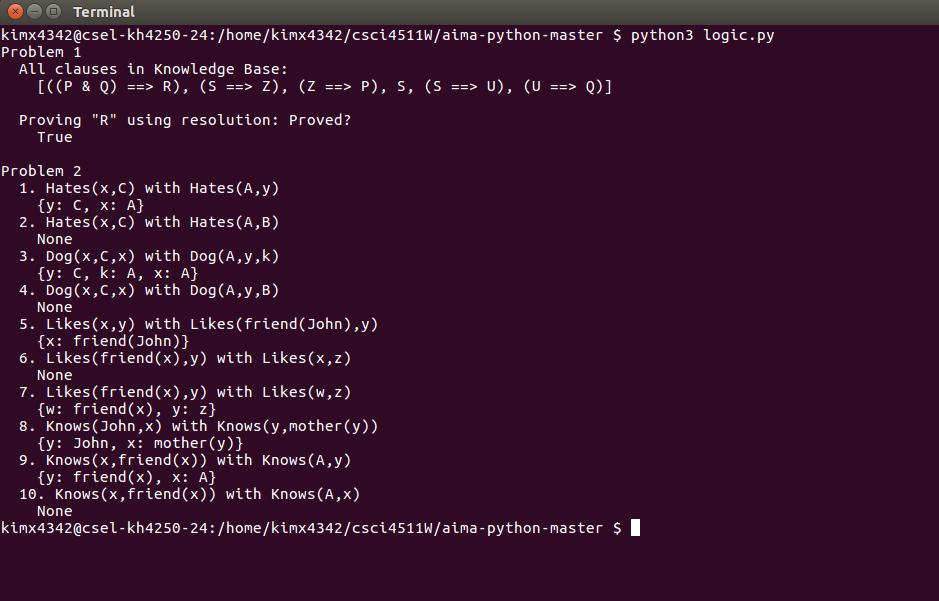
\includegraphics[width=\textwidth]{hw4_1.png}
\end{enumerate}
\end{document}
